%************************************************
\chapter{High Energy Physics at the LHC}\label{ch:plhc} % $\mathbb{ZNR}$
%************************************************

\section{The LHC}

The Large Hadron Collider (LHC) is a circular proton-proton accelerator, located at
CERN, on the Swiss-French border. It is currently the largest and most powerful
particles accelerator ever built. The LHC is built inside the tunnel previously used
for the Large Electron-Positron Collider (LEP). The tunnel is about 27 km in length,
it is located about 100 m underground and the circle rests on a plane inclined
at 1.4$\%$ respect to gravity. In the following we describe the most important features of its design, along with those of the CMS experiment, with \cite{Giannini:2730094} and \cite{Mandorli:2775677} as our main references.

\paragraph{Design and relevant characteristics}

The LHC tunnel has not exactly a circular shape but is formed by 8 rectilinear sections and 8 circular portions. Each arc has an internal radius of 3.7 km and contains
magnetic dipoles that are used to curve the beams reaching a maximum magnetic
field of 8.33 T. The rectilinear sections in the tunnel are approximately 528 m long and host the collision points as well as a series of utilities: magnetic quadrupoles in order to compensate the transverse dispersion of the
protons in the bunches, caused by their mutual repulsion and by synchrotron radi-
ation; radiofrequency cavities, beam injectors and dump facilities.


Four major experimental insertions are located in the rectilinear section. ATLAS (A Toroidal
LHC Apparatus) and CMS (Compact Muon Solenoid) are both multi-purpose experiments, designed to
investigate a wide range of scenarios. Their focus includes Higgs boson properties
study and new physics properties searches at TeV scale. They have similar structures and similar subdetectors in order to have comparable results and to have the
possibility to cross check each other’s studies. ALICE (A Large Ion Collider Experiment) studies a phase of matter called quark-gluon plasma that is formed in
high energy nuclear collisions. Those studies are performed collecting heavy-ion
collisions. LHCb is an experiment designed to perform precision measurement of processes related to b-quark and CP-symmetry violation. Figure \ref{fig:cernacc} shows the entirety of the CERN accelerator complex

\begin{figure}
    \centering
    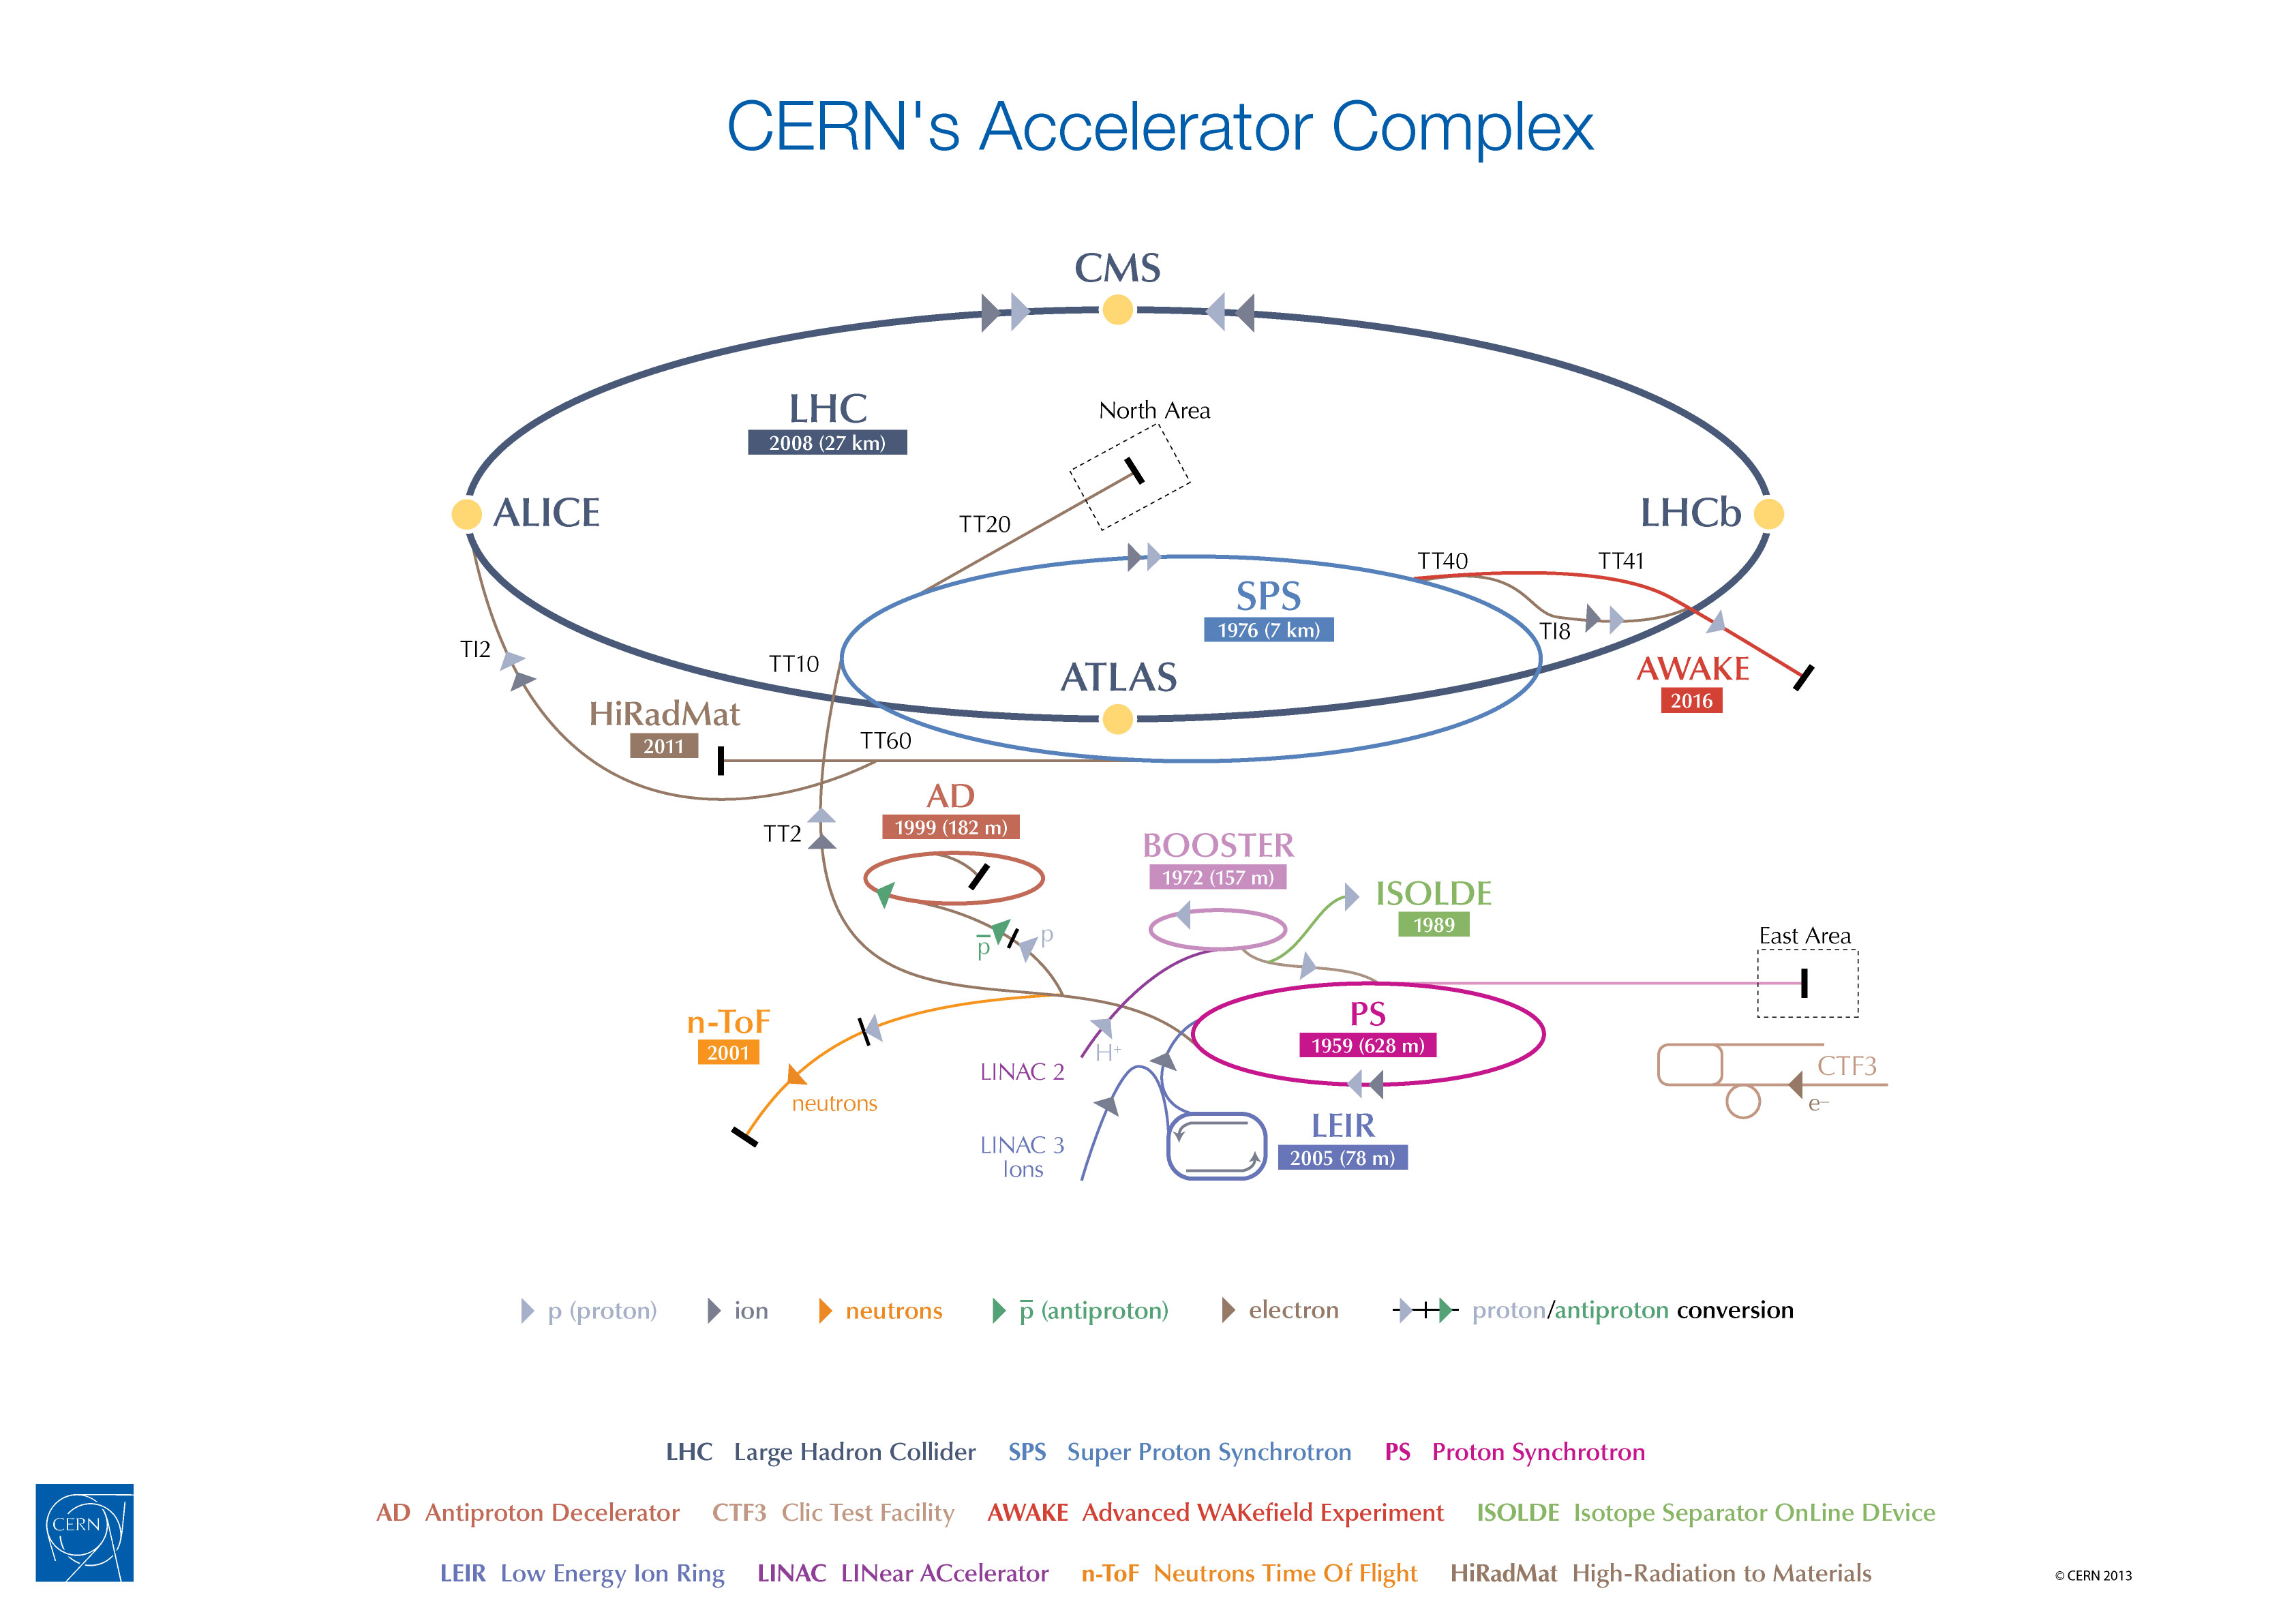
\includegraphics[width=\columnwidth]{gfx/ch1/CERN's-accelerator-complex2013.jpg}
    \caption[The LHC]{To understand the basic design, we show here the LHC along with its accelerator complex. From \cite{acccomplex}.}
    \label{fig:cernacc}
\end{figure}

Protons are accelerated and injected in the LHC by a chain of four accelerators.
The first one is a linear accelerator that injects particles in a chain of three circular
accelerators. Finally, they are injected in the LHC with opposite directions in
two separate beam pipes with an energy of 450 GeV. The particles are accelerated
inside LHC by \emph{radio-frequency cavities} from 450 GeV to a desing-energy of 7 TeV, therefore
the center of mass energy of particles collision is nominally 14 TeV. They circulate
grouped in \emph{bunches}; each beam pipe contains about 2800 bunches in LHC and each
proton bunch has $\approx 10^{11}$ protons. The bunches are spaced 25 ns in time in the nominal
design therefore collisions happen every 25 ns, for a final event rate of about 40 MHz.

\paragraph{Luminosity and pile-up}

The collision rate of an accelerator is measured by its \emph{luminosity}. It's a measurement of the number of collisions that can be produced in a detector per cm$^{2}$ and per second. The bigger is the value of L, the bigger is the number of collisions, making L a key parameter in the design of an accelerator.
Semi-qualitatively, if we define N$^2 \approx (1.15\cdot10^{11})^2$ as the square of the number of protons per bunch, $t$ = 25 ns as the time between bunches and $S_{eff} = 4\pi\sigma$ as the \emph{effective section of collision}, depending on the transversal size of the bunch at Interaction Point ($\sigma \approx 16 \; \mu$m), we obtain L as:

\[ \text{L} = \frac{N^2}{tS_{eff}} \approx 10^{34} \; \text{cm}^2 \text{s}^{-1}
\]

A related quantity is the \emph{integrated} luminosity, which is simply defined as the integral of the luminosity over time.

Searching rare events requires a large number of collisions; for this reason, the
beams are \emph{compressed} in the transverse plane just before entering in the experiments, in order to increase the luminosity of each bunch crossing. Rare events searches need high luminosity, but at high luminosity the rate
of minimum bias collisions exceeds the
bunch crossing rate and there is more
than one minimum bias interaction per
bunch crossing. This effect is known
as \emph{pile-up}. Pile-up interactions produce noise and tracks that make object
reconstruction more difficult, therefore
a compromise has to be found: the higher
the luminosity, the rarer the events that can
be searched, but simultaneously we also have a worse event reconstruction.

\paragraph{Reference frame}

%\begin{figure}
    %\centering
    %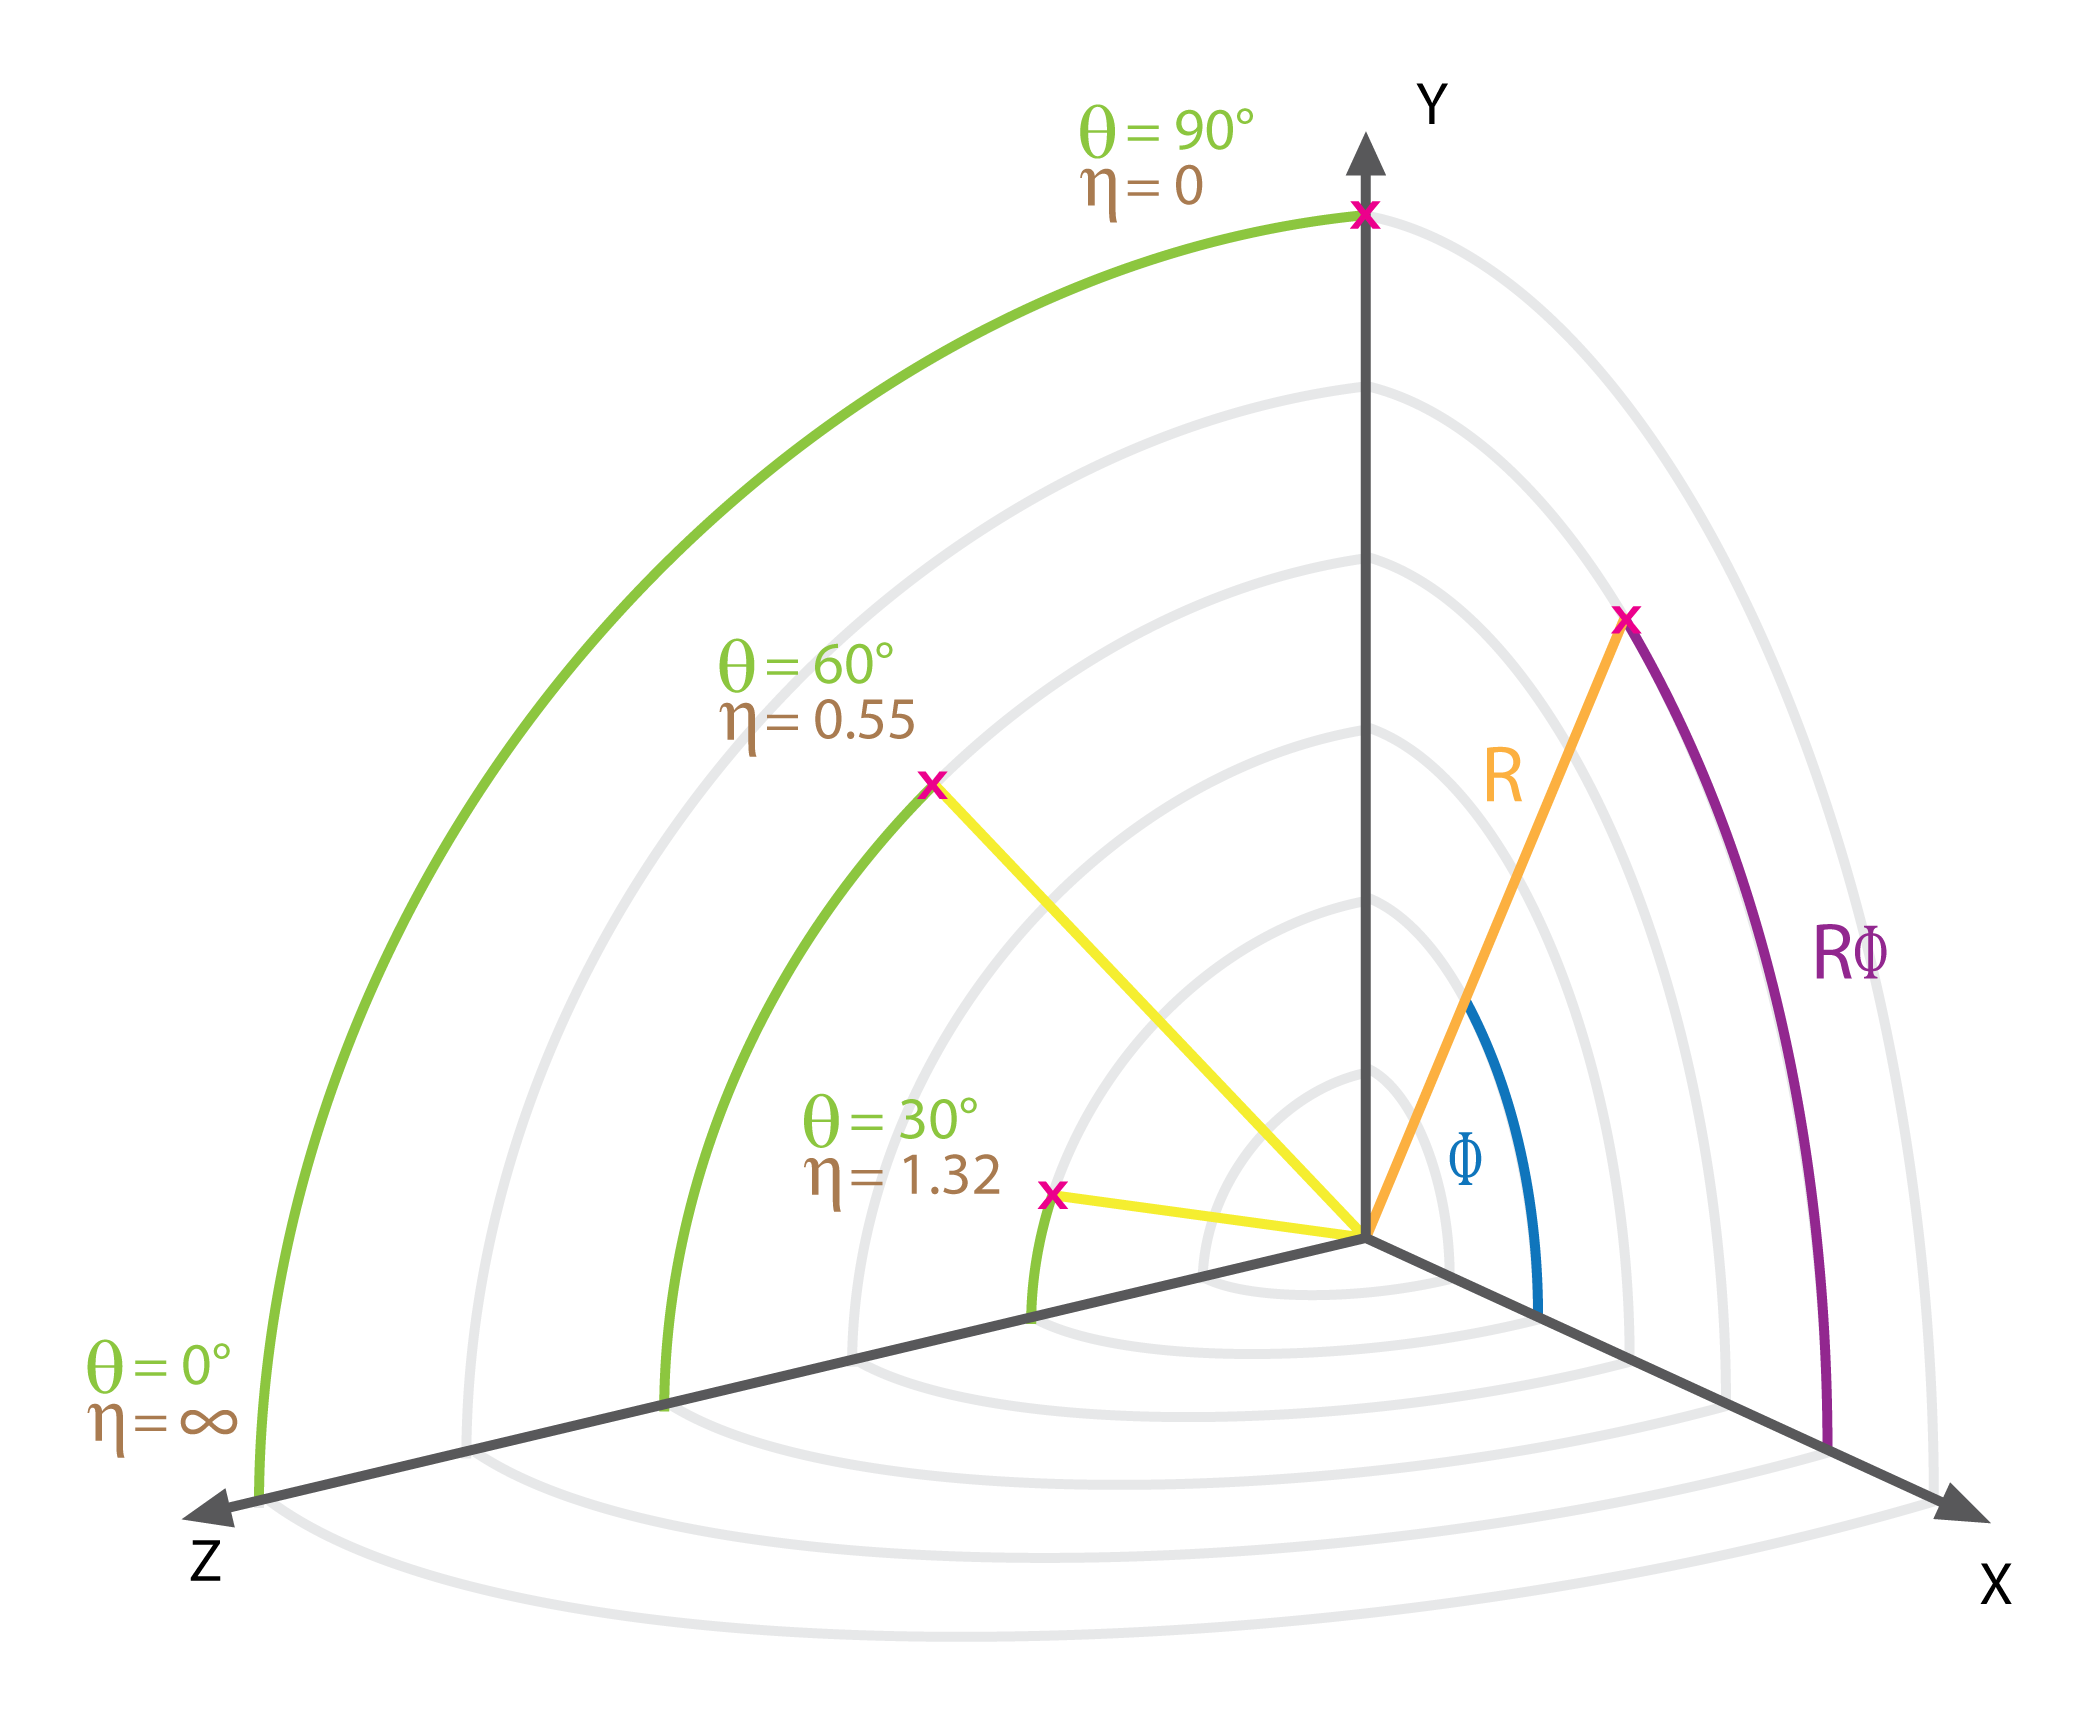
\includegraphics[width=\columnwidth]{gfx/ch1/img_cms_coordinates.png}
    %\caption[Reference frame]{The reference frame at LHC. The z-axis is pointing along the beam %direction. Taken from \cite{Lenzi:1551944}.}
%    \label{fig:reff}
%\end{figure}

The coordinate system used by the experiments at the LHC has its origin fixed at the nominal collision point. The x axis points towards the center of the LHC ring, the y axis points
upwards and the z axis points along the counter-clockwise beam direction. The \emph{azimuthal}
angle $\phi$ is measured from the positive x direction in the xy plane and the \emph{polar} angle $\theta$ is
measured from the positive z direction. The coordinate R usually indicates the distance from
the beam line (R $= \sqrt{x^2 + y^2}$)

In a typical collision, the center-of-mass of the interaction process is boosted along the
z axis with respect to the laboratory frame. The kinematics of the collision products are
therefore conveniently described by the coordinates ($p_T$ , $\eta$, $\phi$, $m$). Here, $\phi$ indicates the
azimuthal angle, $m$ the invariant particle mass and $p_T$ the transverse momentum given by $p_T =
p\sin\theta = \sqrt{p_x^2 + p_y^2}$. Letting $y$ denote the \emph{rapidity}, defined as:

\begin{equation*}
    y = \frac{1}{2}\ln(\frac{E + p_z}{E - p_z})
\end{equation*}

we note that the transverse momentum, the azimuthal angle and the mass are invariant under boosts
along the z direction, while the rapidity is simply additive. The difference in rapidity between two particles is therefore invariant under boosts along the z direction.
The rapidity can however be approximated for ultra-relativistic particles by the \emph{pseudo-rapidity} $\eta$:

\begin{equation*}
    \eta = \frac{1}{2}\ln(\frac{\abs{p}+ p_z}{\abs{p} - p_z}) = -\ln(\tan\frac{\theta}{2}) 
\end{equation*}

which is computed using just the polar angle $\theta$ and is invariant under change of reference frame.

\section{The CMS Experiment}

The Compact Muon Solenoid (CMS) is a barrel shaped detector, centered at the
nominal point where the beams collide. It consists of a central part, called \emph{barrel},
and two external parts called \emph{endcaps}, placed at the ends of the cylindrical barrel.

CMS is a complex apparatus composed of many \emph{subdetectors}--it is illustrated in Figure \ref{fig:cms}.

\begin{figure}
    \centering
    \includegraphics[width=\columnwidth]{gfx/ch1/cms_160312_02.png}
    \caption[CMS]{An at-glance explanation of the CMS experiment and its main components for referencing future discussions. From \cite{decmod}.}
    \label{fig:cms}
\end{figure}

The key feature of CMS is its superconducting solenoid that provides a magnetic field of
3.8 T with the axis aligned along the beams direction. The bore is 13 m long and
it has a radius of 3 m. The magnetic flux is returned by an iron yoke composed by
5 wheel in the barrel and three disk in each endcaps. The strong magnetic flux ensures enough bending power to measure the momentum of the highly energetic muons that
cross the detector.

Starting from the interaction point a particle crosses the\emph{ silicon tracker}, the \emph{electromagnetic calorimeter} (ECAL) and the \emph{hadron calorimeter} (HCAL) before reaching
the solenoid. Outside the coil the \emph{muon detection system} is inserted in the iron of the
yoke of the magnet.

\subsection{Design}

What follows is a brief description of the major subdetectors. As the technical details of each subdetector are extremely subtle, they have already been studied and discussed in numerous articles and are not the focus of our study, we will not discuss them in the present work. The interested reader can found a detailed reference here \cite{Collaboration_2008}. Several upgrades have already been performed during the operational history of the detector, and more are to come in preparation for the \emph{High Luminosity} phase of the LHC.

\paragraph{Tracker}

The tracker constitutes the inner part of CMS and is designed to provide a precise
and efficient measurement of the charged particle \emph{tracks}, i.e. their curvature in the magnetic field, and of the primary and secondary
interaction vertices. It is immersed in an almost homogeneous magnetic field of 3.8 T provided by the CMS solenoid.

A \emph{silicon pixel detector} is installed in the inner region, closest to the interaction point, while \emph{silicon
microstrip detectors} are used in the outer region. The total length of the tracker is 5.8 m
and its diameter 2.5 m, and the angular coverage reaches up to $\abs{\eta}$ = 2.5. 

\paragraph{Calorimeters}

The calorimeters are located outside the tracker and inside the magnetic solenoid. They are
designed to measure the energy of electromagnetic and hadronic showers and, unlike the
tracker, they are required to completely absorb the particles in the shower for optimal energy measurements. They are therefore required to be \emph{heavy}, which translates into a large
number of radiation lengths $X_0$ for the ECAL and of interaction lengths $\lambda_I$ for the HCAL.
The full tracker material has a thickness of $\approx$ 0.5-1 $X_0$ and less than one $\lambda_I$ for comparison.

\begin{outline}
    \1 The ECAL is a homogeneous calorimeter made
    of 61200 PbWO4 crystals mounted in the central barrel part, completed by 7324 crystals in
    each endcap. The ECAL barrel covers the central rapidity region ($\abs{\eta}$ < 1.48) and the two
    ECAL endcaps extend the coverage up to $\abs{\eta}$ = 3. A lead/silicon-strip preshower detector is
    also installed at pseudorapidities 1.6 < $\abs{\eta}$ < 2.6. The crystals are all active material: they
    induce the shower and generate scintillation light to measure the shower energy. The scintillation light is detected by silicon avalanche photodiodes in the barrel region and vacuum
    phototriodes in the endcap region. 
    
    The typical \emph{energy reslution} is:
    
    \begin{equation*}
        \frac{\sigma_E}{E} = \frac{a}{E} + \frac{b}{\sqrt{E}} + c
        \end{equation*}
        
    where a $\approx$ 0.12 GeV is the noise term due the electronics and pileup, independently of the energy, b $\approx$ 2.8$\%$ is
    the stochastic term which accounts mainly for the fluctuations in the photon conversions,
    and c $\approx$ 0.3$\%$ is a constant term related to the energy scale calibration.
    
    \1 The HCAL is used to measure the energy of hadrons, and it
    is the only detector available to measure the energy of stable neutral hadrons. Its design ensures
    good hermeticity to allow the measurement of the missing transverse energy and angular
    coverage in the forward region for forward jets.
    Four regions are instrumented with HCAL detectors: the barrel hadron calorimeter (HB)
    surrounds the electromagnetic calorimeter and covers the central pseudorapidity region up
    to $\abs{\eta}$ = 1.3; the two endcap hadron calorimeters (HE) cover up to $\abs{\eta}$ = 3. The Cherenkov-based, Hadronic-forward
    calorimeter (HF) extends the coverage up to $\abs{\eta}$ = 5 in the forward region. An array of scintillators, the outer hadron calorimeter (HO), is located outside the magnet to catch the tails
    of the hadronic shower and avoid the misidentification of muons. Contrary to ECAL, the HCAL is a sampling calorimeter: the energy is measured by scintillators alternated to brass plates used as absorbers in HB and HE.
    
    The HCAL is coarser than the ECAL and the resolution is also worse:
     the combined ECAL+HCAL resolution measured in a pion test
    beam was $\sigma_E /E = 110\%/\sqrt{E} + 9\%$.
\end{outline}

\paragraph{Muon chambers}

The muon system is located outside the solenoid and covers the pseudorapidity range
$\abs{\eta}$ < 2.4. Outside of the solenoid coil, the magnetic field flux is returned through a steel
yoke. Three steel layers are present both in the barrel and in the endcaps, alternated with
four layers of muon detectors.


The muon system provides information to identify muons and to measure the momentum
and charge of high-$p_T$ muons. Additionally, two tasks are accomplished by the muon system thanks to its good time resolution: \emph{bunch crossing} identification and \emph{muon-triggering}.
Three different gaseous detector technologies are used: \emph{drift tube} (DT) chambers and \emph{cathode strip} chambers (CSC), supplemented by a system of \emph{resistive plate} chambers (RPC). Both the DTs and the CSCs are primarily tracking detectors, but have also
good time resolution. The RPCs instead are mainly used for their good time resolution.


\paragraph{Trigger}

The 40 MHz rate of proton-proton collisions and the pileup make it impossible to process
and store all the information provided by the detector. Most of the events are not interesting
for physics analysis in any case, due the to fact that the total proton-proton cross section
is more than 6 orders of magnitude larger compared to the cross section of interesting processes. The data needs to be reduced and selected trough a trigger system, whose crucial
aspect is a fast and efficient real-time selection to record the useful events.

In CMS the data reduction happens in two steps. The \emph{Level-1} (or L1) Trigger consists of programmable electronic devices, reducing  the event rate from an input of 40 MHz to an output of about 100 kHz. The
\emph{High Level Trigger} (HLT) further decreases the event rate from about 100 kHz to about 1 kHz for data storage. The HLT is implemented by a computer farm composed of more than 30000 CPUs
running software modules similar to the ones used for the offline reconstruction. 

\paragraph{Offiline reconstruction}\label{sec:offreco}
Once the event has been selected by the trigger, other crucial, offline processing aspects are the \emph{track reconstruction}, the \emph{primary vertex reconstruction} and the \emph{particle flow} algorithm for particle identification. These, along with other minor steps, are all needed to transform the electronic outputs of the apparatus into a collection of physical objects needed for the analysis.

\begin{outline}
    \1 The track reconstructions algorithms identify tracks from the single hits in the tracker region. It is an \emph{iterative} algorithm, which is run multiple times starting from easier, non-displaced tracks of higher $p_T$. It has three major steps: \emph{seeding} or initialization, then \emph{pattern matching} to identify possible candidates of a track and \emph{track fitting} to identify the most convincing candidate tracks.
    
    The tracking efficiency saturates at $\approx$ 90 $\%$ due to hadrons that undergo nuclear interactions in the tracker material, while it is known to be close to 100 $\%$for muons. At low $p_T$ the efficiency is lower due to the nuclear interactions;
    
    \1 The particle flow algorithm is capable of transforming the readouts into a list of final state particles produced in the event and their properties. It takes as inputs tracks (also from muon chambers) and caloritmeters clusters, and defines a PF \emph{block} as the building unit of a physical object, defined as a series of links between single hits. Muons, electrons and isolated photons, Jets and their constituents as well as $p_T^{miss}$ are all reconstructed in this step; 
    
    \1 Due to pile-up, we have multiple vertices for each event. The vertex reconstruction steps is responsible for employing the newly found tracks to identify the primary vertex to be used in the analysis. Its action can be quantitatively explained as selecting the vertex with the higher $\sum p_T$ of all the collision products identified by the previous step.
\end{outline}

\paragraph{Luminosity and Pile-up}

 The CMS designed luminosity of 10$^{34}$ cm$^{-2}$ s$^{-1}$ has been achieved and exceeded in the last three years of data taking. Integrated luminosity recorded by CMS and employable for physics analyses are 35.9 fb$^{-1}$ for 2016, 41.53 fb$^{-1}$ for 2017, and 60.0 fb$^{-1}$ for 2018.

As discussed above this also meant an increase in pile-up: Figure \ref{fig:pileup} shows its increase over the various years.

\begin{figure}
    \centering
     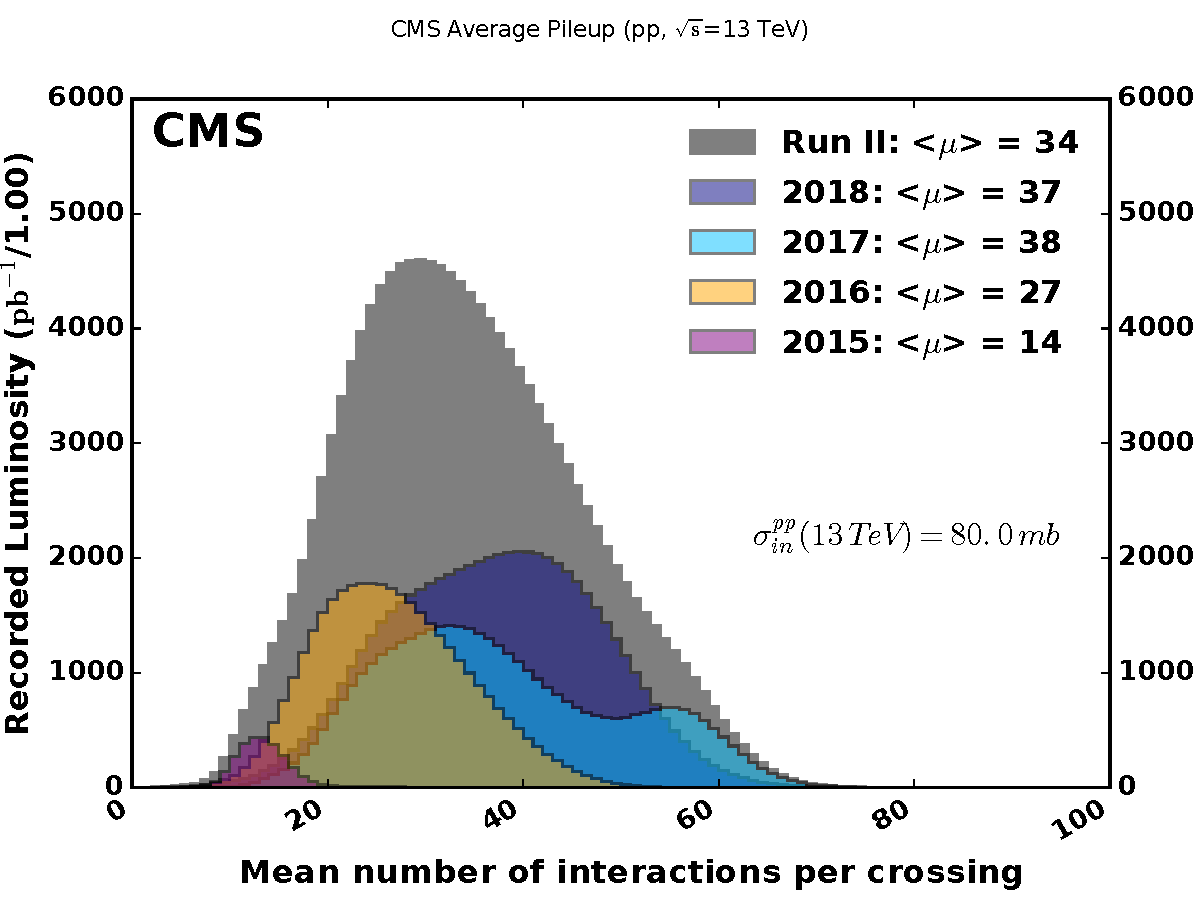
\includegraphics[width=\columnwidth]{gfx/ch1/pileup_allYears_run2.pdf}
    \caption[Pile-up]{The pile-up is greatly increasing over the years--as shown by the distribution of the average number of interactions per crossing for pp collisions in 2011 (red), 2012 (blue), 2015 (purple), 2016 (orange), 2017 (light blue), and 2018 (navy blue). From \cite{cmspubliclumi}.}
    \label{fig:pileup}
\end{figure}

\section{Physics program and measurements}

Being a general-purpose experiment, CMS is capable of performing a wide range of interesting and insightful measurements. Aside from the discovery of the Higgs boson and the study of its couplings, which will be discussed below in greater detail, we mention briefly the other directions of CMS research:

\begin{outline}
    \1 The \emph{SM physics} programme includes all the studies of the LHC data with the goals of measuring fundamental parameters of the Standard Model of particle physics. The cross-sections of a large variety of processes happening during the beam collisions are determined with the best precision possible and compared to the most up-to-date theory calculations, from the most common to the rarest of them all. Fundamental parameters of the theory such as masses of elementary particles and gauge couplings are measured to verify the effectiveness of the predictions, and any deviations of data from the Standard Model are quantified. The various \emph{couplings} expected between particles are investigated in detail. As an example, the \emph{Vector Boson Scattering} is a series of processes such as $W^{\pm} Z \rightarrow W^{\pm} Z$, however, it can admit higher-order couplings to the Higgs boson as $W^{\pm} Z \rightarrow H^{\pm} \rightarrow W^{\pm} Z$ which are to be investigated to compare their productions to what is expected from theory;
    
    \1 The \emph{Top Quark physics} programme consists in the precision measurements of the properties of the top quark, the heaviest particle in the standard model. The top-quark mass is one of the most important properties as it is a key parameter for calculations in the standard model. The top group also aims to establish measurements of rare production modes of the top quark in association with other particles, and search for new couplings of the top quark. It also aims to improve our understanding of top quark production and decay processes in order to improve background predictions as well as providing indirect proof for physics searches beyond the standard model;
    
    \1 \emph{Supersymmetry (SUSY), Exotica} and \emph{Beyond-Two-Generations} are a collection of groups working on generic processes beyond the SM predictions. SUSY consists in the search for physics signatures involving large missing transverse momentum, together with other features such as jets, muons, electrons, taus, photons, and b-jets. If we discover such signatures with yields significantly in excess of standard model backgrounds, our goal will be to characterize the event samples as fully as possible, as possible evidence of a supersymmetric theory. Exotica includes all the other processes not related to SUSY, while the B2G group covers models of new physics featuring the decay of new resonances to heavy standard model objects such as top, W, Z, or Higgs bosons. In particular, they study exotic \emph{diboson} resonances, partners of the top quark with vector-like properties (VLQ) as well as heavy resonances, such as W' and Z' resonances decaying to final states with top quarks.;
    
    \1 Finally, the \emph{B physics} group addresses all the heavy flavor (beauty and charm) studies. These activities involve precision measurements of heavy-quark hadron production, decay and properties, and the search for associated new and rare processes;
    
\end{outline}

\subsection{The Higgs discovery and searches}

The main driver for the construction of the LHC and the deployment of the CMS experiment is certainly the Higgs boson and the detailed study of its properties. 

The Higgs is a \emph{scalar boson}, i.e. with spin $0$, whose presence in the theory is needed in order to explain the masses of the \emph{gauge bosons} (as well as the fundamental fermions) through the \emph{Higgs mechanisms}: a spontaneous symmetry breaking of the scalar fields embedded in the U(1)$\times$SU(2) local gauge symmetry of the electroweak sector. The mass of the Higgs particle is a \emph{free parameter} of the theory. The Higgs boson is also expected to  interact with the entire fermion sector trough \emph{Yukawa}-like vertices, with a coupling proportional to the fermion mass.

The Higgs boson, which is consistent with the SM Higgs according to the current experimental data, was discovered in 2012 at the LHC (see \cite{Aad_2012} and \cite{Chatrchyan_2012}). The mass of the new particle, approximately 125 GeV, sets the boundaries of today well-know Higgs phenomenology.

After having established the mass of the newly-observed boson, along with its major couplings during Run 1, both ATLAS and CMS renewed their efforts to improve the previous results and investigate the couplings of the Higgs to the fermions through Run 2 data. The most recent results published for the branching ratio signals are showed in Figure \ref{fig:sigsm}.

\begin{figure}
    \myfloatalign
    \subfloat[]
    {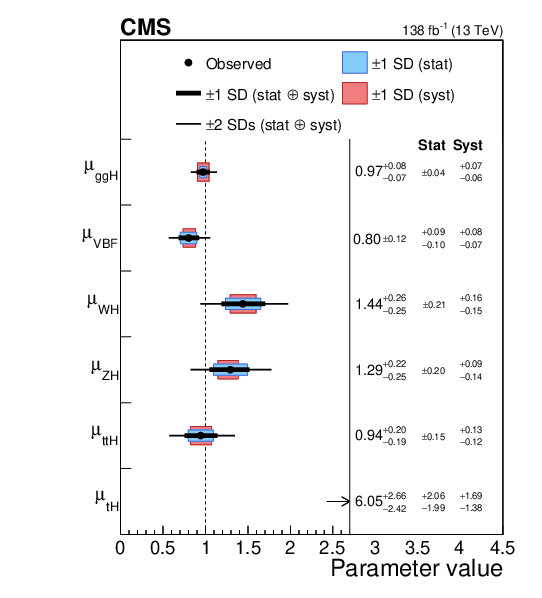
\includegraphics[width=.465\linewidth]{gfx/ch1/Figure_002-a.png}} \quad
    \subfloat[]
    { 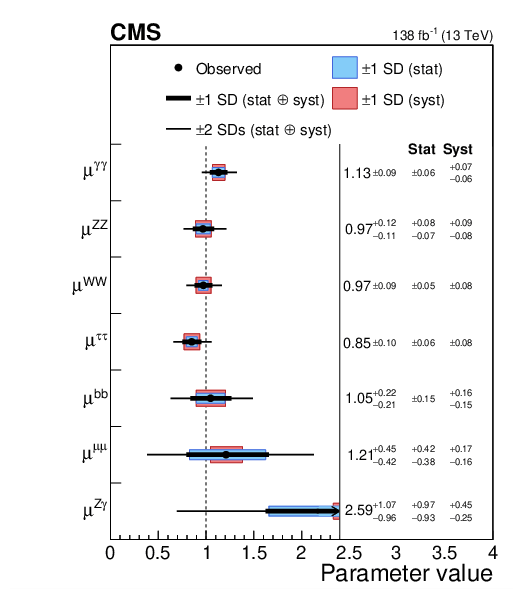
\includegraphics[width=.45\linewidth]{gfx/ch1/Figure_002-b.png}} \\
    \caption[Signal strength modifiers]{A fundamental example of the CMS research results: the summary plots showing the measured signal strength per
    production mode at $\sqrt{s}$ = 13 Tev (a) and the measured signal
    strength per decay channel at $\sqrt{s}$ = 13 Tev (b). Taken from \cite{higgsrevcms}}\label{fig:sigsm}
\end{figure}

They are expressed as the \emph{signal strength modifier} $\mu$, a ratio between the observed value and  the SM prediction, defined as:

\[
\mu_P = \frac{\sigma_i}{\sigma_{i, SM}} \quad \mu^D = \frac{\text{BR}_i}{\text{BR}_{i, SM}}
\]

where we have distinguished between the \emph{production} and \emph{decay} modifiers, and $\mu = \mu_P \cdot \mu^D$.

During Run 3, which is just starting at the time of writing, the
physics of the Higgs boson at the LHC is entering a time of precision measurements and
search for rare decays. Highly precise measurements are a powerful test for the theoretical predictions of the SM: small but significant deviations could appear which may hint at physics beyond our current theoretical description.

\subsection{The VBF Channel of H$\rightarrow\mu^+\mu^-$ as a benchmark for simulation}\label{sec:targets}

\begin{figure}
    \myfloatalign
    \subfloat[]
    {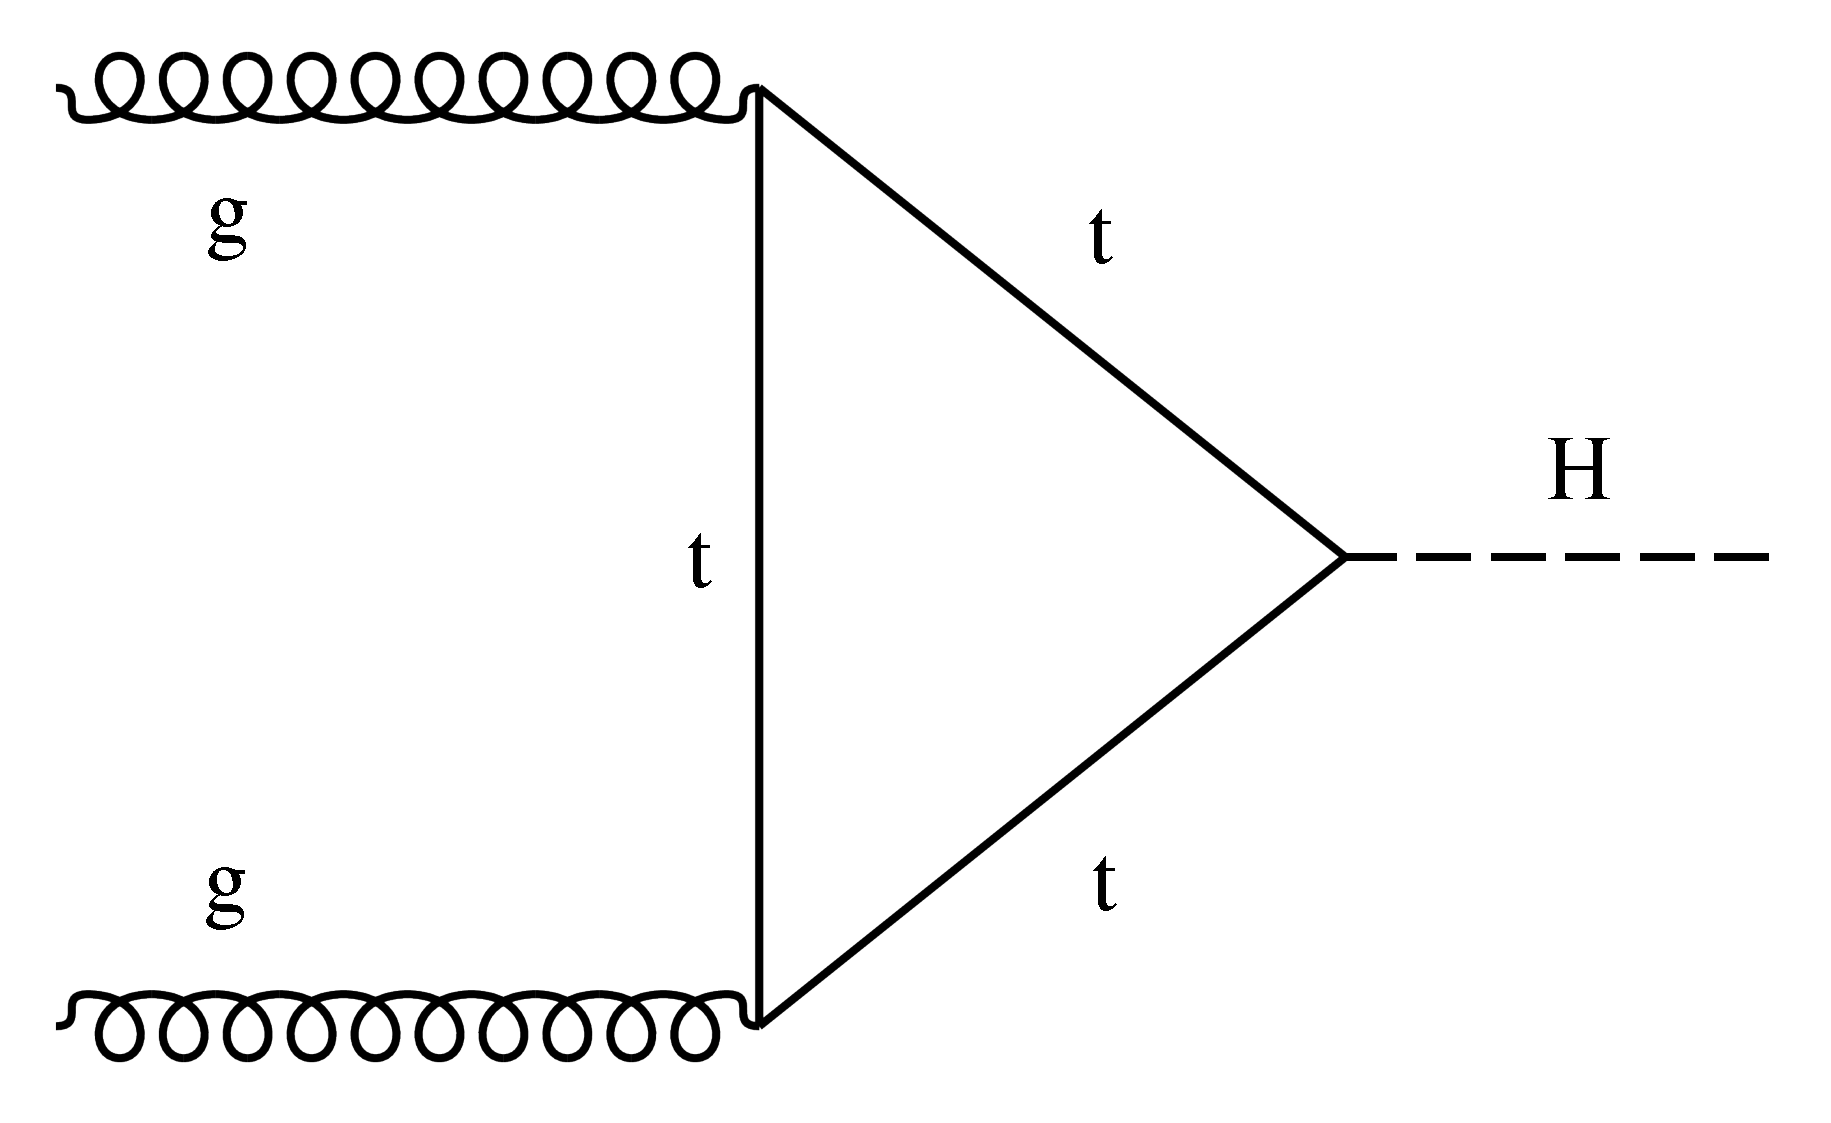
\includegraphics[width=.45\linewidth]{gfx/ch1/CMS-HIG-17-031_Figure_002-a.pdf}} \quad
    \subfloat[]
    { 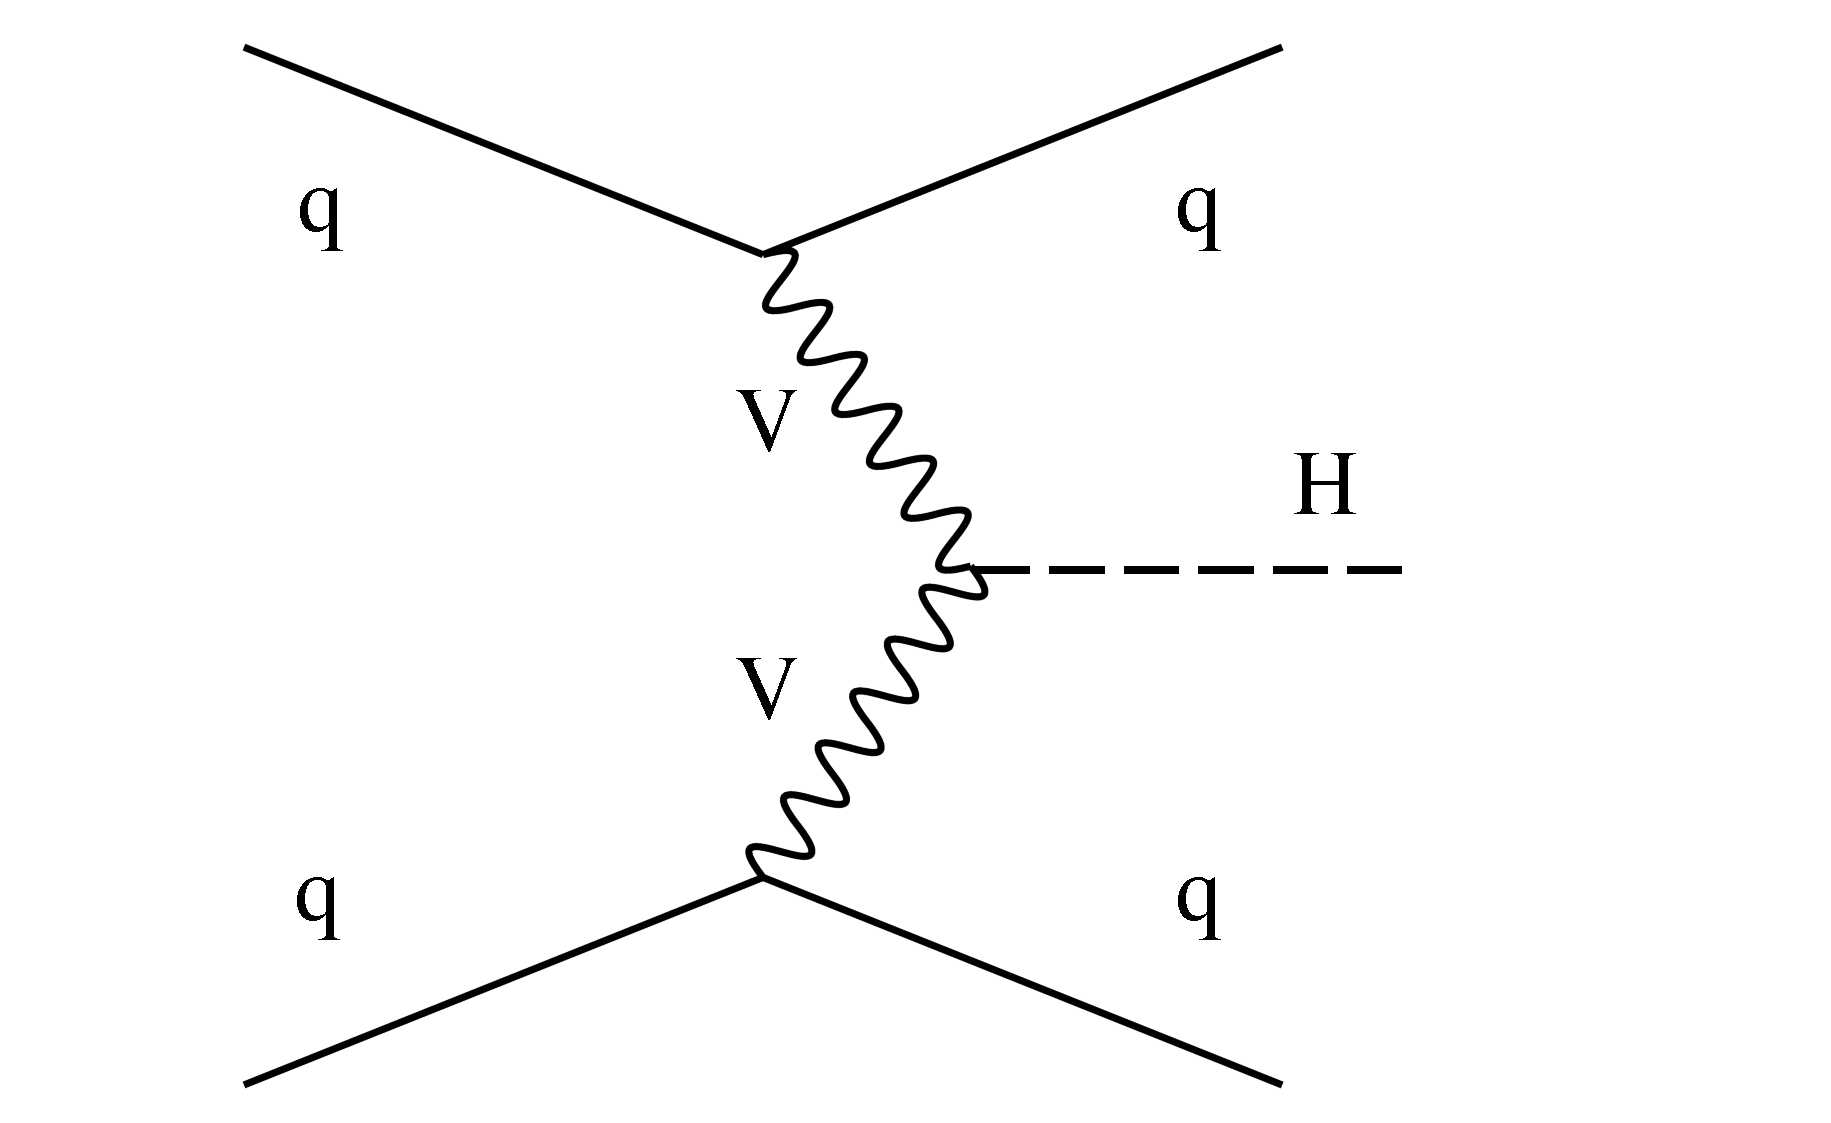
\includegraphics[width=.45\linewidth]{gfx/ch1/Figure_001-b.pdf}} \\
    \caption[ggF and VBF]{Leading Feynman diagrams for Higgs boson production via ggF (a) and VBF (b), the one central to our discussion.}\label{fig:feypro}
\end{figure}
Having discussed the importance of the Higgs studies, we now present a specific production channel, as well as the two muon decay, explaining why they will serve as a solid benchmark for our deep learining approach to simulation.

In the SM, the phenomenology of the Higgs boson decays depends crucially on its mass,
which defines the branching fractions. The production modes instead have a milder Higgs
mass dependence. In proton-proton collisions at the center-of-mass energies currently reached by the LHC
(up to 13 TeV) four main production mechanisms are expected. The gluon-gluon fusion
production mode has the largest cross section, followed by vector boson fusion, associated
WH and ZH production, and production in association with a t$\overline{\text{t}}$  or b$\overline{\text{b}}$ pair. The gluon-gluon fusion (ggF) is the dominant production mode with a cross section of
approximately 85$\%$ of the total. The leading diagram involves a quark loop, given the fact that the H does not directly couple with massless gluons: the main
contribution to the SM amplitude arises from the top quark loop, though the amplitude is
potentially sensitive to the presence of new massive particles with non zero color charge.

The vector boson fusion (VBF) has a cross section of about a tenth of the gluon-gluon fusion one. The leading diagrams involve a qq scattering, with a
vector boson exchange and the emission of a Higgs boson. Since the momentum exchange
is typically lower than the center-of-mass energy of the two quarks, the channel is characterized by two separated high-rapidity quarks in the final state, detectable as high rapidity
jets. Their presence can therefore serve as a signature of the VBF production channel. Additionally, as VBF is a pure electroweak process, low hadronic activity is expected in the
rapidity gap between the two jets, where the Higgs decay products are typically found. The Feynman diagrams for the two dominant production processes are showed in Figure \ref{fig:feypro}. Experimentally, the signal over background ratio for the VBF channel is higher than that for other production modes, thanks to its key characteristics: few, energetic jets, highly energetic muons, a large rapidity gap.

This production mode is also an ideal candidate for our FlashSim simulation approach, for a series of reasons:

\begin{itemize}
    \item The building blocks of the analysis are mainly the jets and the muons, meaning that to perform a comparison we will need to simulate a smaller number of physical objects when compared to other channels;
    \item The physical analysis is actually Monte Carlo-based, meaning that it is possible to validate our samples by comparing them to ones from the conventional simulation pipeline which have already been produced;
    \item A greater amount of MC-data would benefit the analysis by allowing a more accurate background modelling;
    \item Additionally, a flash simulation approach could also address the need for computing several different theoretical variations;
    \item More generally, due to the expected increase in luminosity during Run 3, the need for MC samples will also increase.
\end{itemize}

The Pisa CMS Group worked extensively on the VBF Channel for the publication of \cite{CMS-PAS-HIG-19-006}, allowing us to take advantage of the expertise and insights of the group.
Because of this, in the latter part of this work we will compare the original samples employed in \cite{CMS-PAS-HIG-19-006} with the ones obtained through our approach.
At the time of writing, the CMS collaboration has managed to provide evidence of the H$\rightarrow\mu^+\mu^-$ up to 3$\sigma$ (see \cite{Sirunyan_2021}) Some relevant plots are shown in Figure \ref{fig:vbfmm}.

\begin{figure}
    \myfloatalign
    \subfloat[]
    {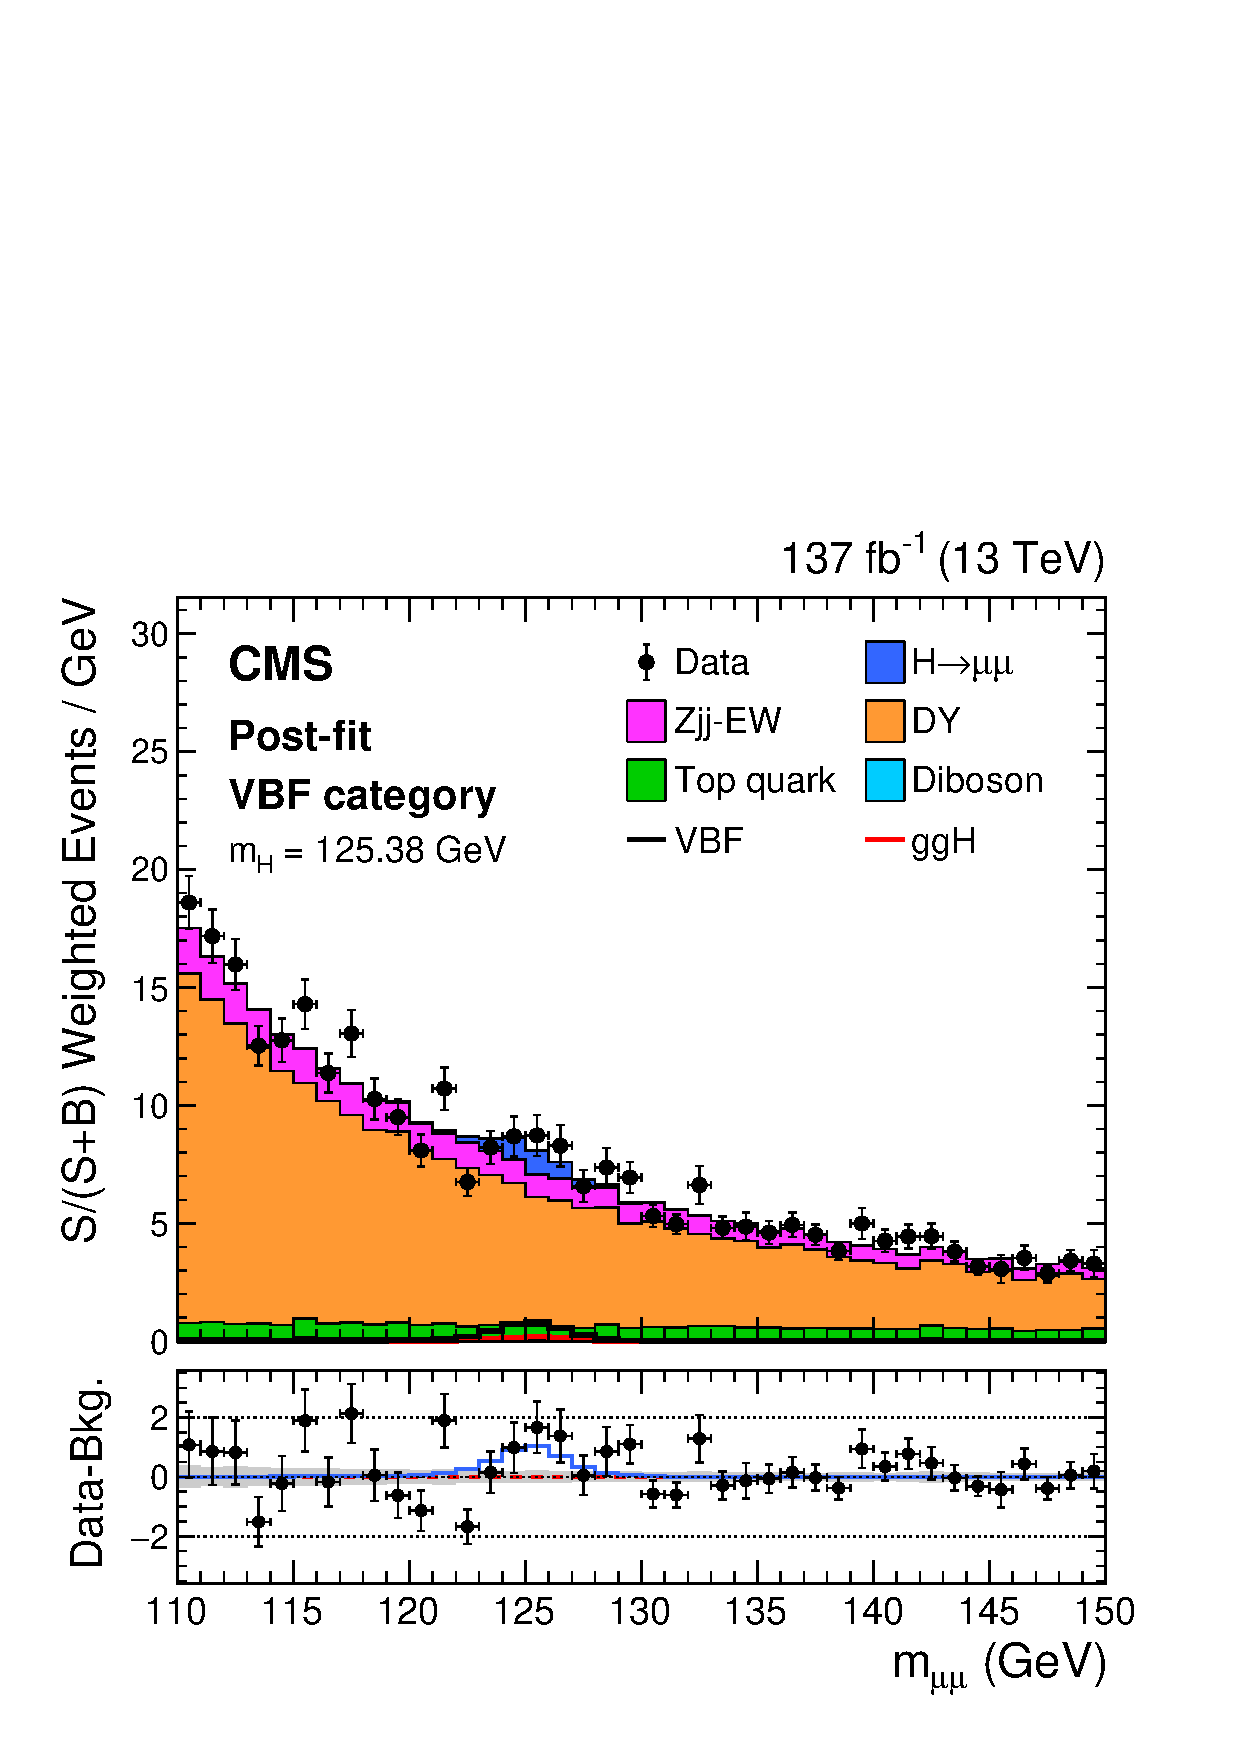
\includegraphics[width=.45\linewidth]{gfx/ch1/CMS-HIG-19-006_Figure_012-a.pdf}} \quad
    \subfloat[]
    { 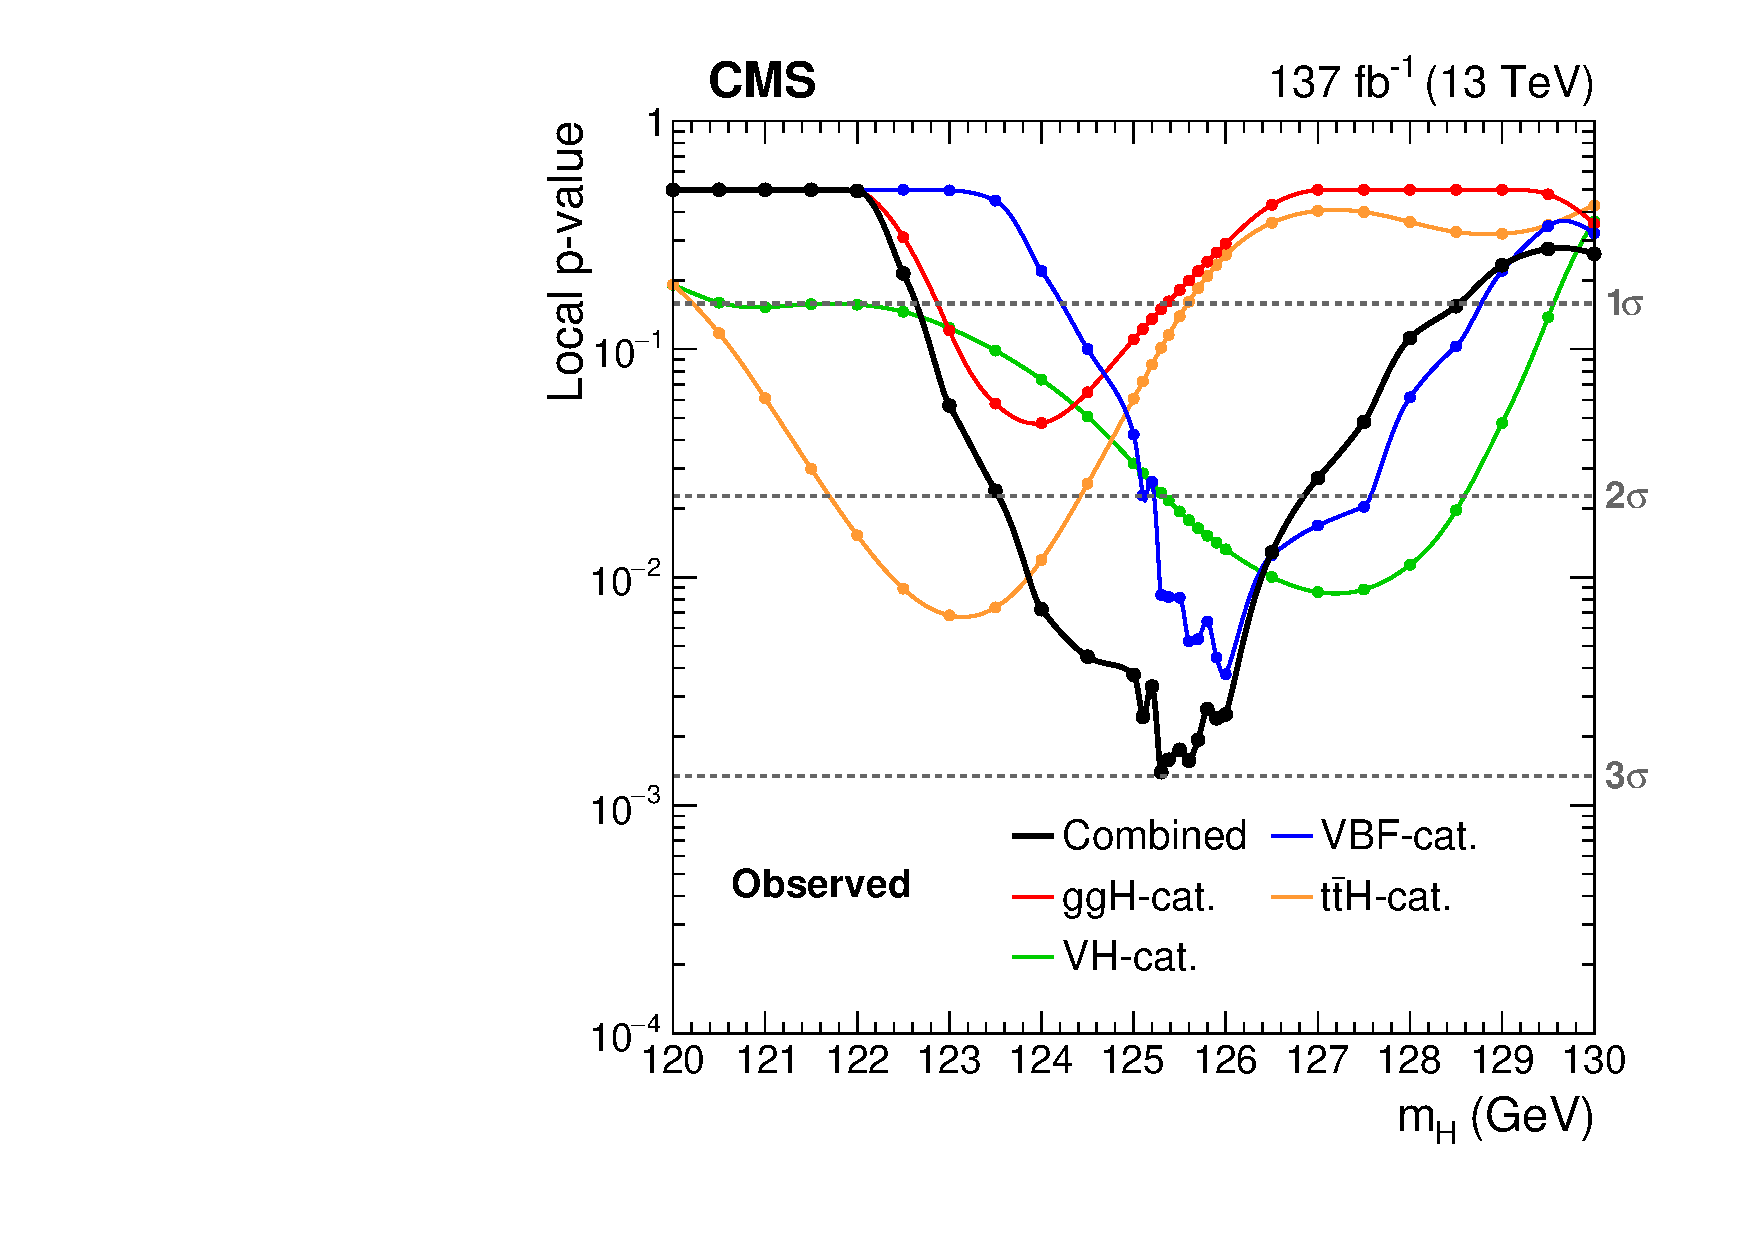
\includegraphics[width=.45\linewidth]{gfx/ch1/CMS-HIG-19-006_Figure_010-a.pdf}} \\
    \caption[H$\rightarrow\mu^+\mu^-$]{You can observe that, thanks to its clear signature, the VBF channel is the one providing the greatest evidence around the Higgs mass region: (a) The $m_{\mu\mu}$ distribution for the weighted combination of VBF-SB and VBF-SR events (the lower panel shows the residuals). (b) Observed local p-values as a function of $m_H$. From \cite{Sirunyan_2021}.}\label{fig:vbfmm}
    
\end{figure}

Other possible processes which we could have chosen for comparison, and which would surely benefit from a flash production of samples due to similar reasons as before, are the H$\rightarrow$bb decay as well as the ttH production mode. However, as we are presenting a \emph{proof-of-concept}, we decided to stick to the VBF channel as it present the unique advantage of needing simulations for just the jets and the muons, as opposed to the other candidates. 